%  Autores: Giuliano Crenna · Bruno Emanuel Pace
%  Compilar con: pdfLaTeX (recomendado en Overleaf)

\documentclass[12pt,a4paper,spanish]{article}

\usepackage[utf8]{inputenc}
\usepackage[T1]{fontenc}
\usepackage[spanish,es-tabla]{babel}
\usepackage[margin=2.5cm]{geometry}
\usepackage{graphicx}
\usepackage{xcolor}
\usepackage{hyperref}
\usepackage{enumitem}
\usepackage{booktabs}
\usepackage{array}
\usepackage{caption}
\usepackage{float}
\usepackage{fancyhdr}
\usepackage{url}
\usepackage[nottoc]{tocbibind}
\usepackage{setspace}
\usepackage{pgfgantt}        % Diagrama de Gantt para el cronograma
\usepackage{colortbl}        % Colorear celdas de tablas
\usepackage{tabularx}        % Tablas con ancho controlado
\onehalfspacing

\definecolor{ugrAzul}{HTML}{0B3D91}   
\definecolor{ugrCeleste}{HTML}{3FA9F5}
\definecolor{ugrVerde}{HTML}{2E8B57}
\definecolor{ugrNaranja}{HTML}{E07B00}
\definecolor{ugrVioleta}{HTML}{6A4C93}
\definecolor{ugrGris}{HTML}{7A7A7A}

\hypersetup{
    colorlinks=true,
    linkcolor=blue!60!black,
    citecolor=blue!60!black,
    urlcolor=blue!60!black,
    pdftitle={Detección temprana de depresión mediante lenguaje},
    pdfauthor={Giuliano Crenna · Bruno Emanuel Pace}
}

\pagestyle{fancy}
\fancyhf{}
\fancyhead[L]{\small Proyecto de Trabajo Final}
\fancyhead[R]{\small Crenna, Pace}
\fancyfoot[C]{\thepage}
\renewcommand{\headrulewidth}{0.4pt}
\setlength{\headheight}{14pt}

\begin{document}

\begin{titlepage}
    \centering
    \vspace*{0.3cm}
    {\large \textbf{Universidad del Gran Rosario}\par}
    \vspace{0.2cm}
    {\large \textbf{Área de Tecnología y Negocios}\par}
    \vspace{0.4cm}
    
\includegraphics[width=0.60\textwidth]{logo_ugr.png}\par
    \vspace{0.6cm}
    {\Large \textbf{PROYECTO DE TRABAJO FINAL}\par}
    \vspace{0.2cm}
    {\Large \textbf{Seminario de Trabajo Final}\par}
    \vspace{0.7cm}
    \rule{0.85\textwidth}{0.6pt}\par
    \vspace{0.4cm}
    {\LARGE \textbf{Detección temprana de depresión mediante procesamiento de lenguaje natural y aprendizaje automático}\par}
    \vspace{0.3cm}
    \rule{0.85\textwidth}{0.6pt}\par
    \vspace{0.8cm}

    {\large \textbf{Autores:}\par}
    \vspace{0.2cm}
    {\large Tec. Univ. Giuliano Crenna\quad --\quad \textbf{DNI 43.841.488}\par}
    \vspace{0.15cm}
    {\large Tec. Univ. Bruno Emmanuel Pace\quad --\quad \textbf{DNI 43.127.593}\par}
    \vspace{0.8cm}
    {\large \textbf{Lugar:} Rosario, Santa Fe, Argentina\par}
\end{titlepage}

\pagenumbering{roman}
\setcounter{page}{2}

\section*{Resumen}
\addcontentsline{toc}{section}{Resumen}

En el presente trabajo se propone el desarrollo de un sistema de detección temprana de depresión a partir del análisis automático de texto, empleando técnicas de Procesamiento de Lenguaje Natural (PLN) y aprendizaje automático supervisado. La motivación central es que los trastornos depresivos constituyen uno de los problemas de salud mental más prevalentes a nivel global —la Organización Mundial de la Salud estima que aproximadamente un 5{,}7\,\% de los adultos los padece~\cite{who2025depression}— y que una proporción significativa de personas expresa indicadores lingüísticos de malestar psicológico en redes sociales y otros canales digitales antes de buscar ayuda profesional~\cite{nature2026review,pmc11574504}. El trabajo plantea construir un corpus en español, entrenar y comparar modelos de referencia (TF-IDF + regresión logística, SVM, BETO) y un modelo transformer afinado para clasificar usuarios con probabilidad alta, media o baja de presentar sintomatología depresiva, prestando especial atención a la interpretabilidad de los marcadores lingüísticos identificados. Como resultado esperado se obtendrá un modelo reproducible, una caracterización de marcadores en español y una evaluación crítica del estado del arte en la materia.

\textbf{Palabras clave:} Procesamiento de Lenguaje Natural; Depresión; Detección Temprana; Aprendizaje Automático; BERT; Salud Mental; Redes Sociales; Español.

\textbf{Temática de interés en Ciencia de Datos:} Aprendizaje Automático Supervisado y PLN aplicado a salud.

\section{Problemática observada}
\addcontentsline{toc}{section}{Problemática observada}

La depresión es un trastorno del estado de ánimo cuya carga mundial sigue en aumento. Las cifras más recientes de la Organización Mundial de la Salud indican que en 2021 alrededor de 332 millones de personas padecían algún trastorno depresivo, que menos del 10\,\% de quienes lo sufren reciben un tratamiento mínimamente adecuado y que la prevalencia es aproximadamente 1{,}5 veces mayor en mujeres que en hombres~\cite{who2025depression,who2025mentalhealth}. La detección tardía se asocia a peor pronóstico, mayor riesgo de suicidio y mayor coste sociosanitario~\cite{jmir2019spanish}.

En paralelo, el uso masivo de redes sociales y mensajería instantánea ha generado un volumen sin precedentes de texto en lenguaje espontáneo en el que muchas personas manifiestan, de forma más o menos explícita, marcadores lingüísticos asociados a estados depresivos: uso elevado de pronombres en primera persona del singular, vocabulario absolutista (``siempre'', ``nada'', ``nunca''), lenguaje absolutista, mayor densidad de emociones negativas, descenso del contenido social y patrones de actividad temporal alterados~\cite{aisel2023mentalbert,jmir2019spanish,pmc8993841,frontiers2025xai}. Esta huella lingüística puede aprovecharse como una señal \emph{temprana} y \emph{no intrusiva} para alertar a un potencial afectado, sin reemplazar el diagnóstico clínico~\cite{leis2019tesis}.

El problema, por tanto, no es sólo clínico sino también computacional y social: ¿es viable construir un modelo que, a partir de texto escrito en español, identifique perfiles con alta probabilidad de presentar sintomatología depresiva, manteniendo una precisión razonable, respetando la privacidad del usuario y siendo interpretable por profesionales de la salud mental?

\section{Hipótesis de investigación}
\addcontentsline{toc}{section}{Hipótesis de investigación}

\textbf{Hipótesis principal.} \emph{Es posible desarrollar un modelo de aprendizaje automático supervisado que, a partir de texto escrito en lengua española y representaciones del lenguaje natural, clasifique usuarios con sintomatología depresiva frente a controles, con un rendimiento superior y estadísticamente significativo respecto a los modelos de referencia clásicos, evaluado mediante una batería multidimensional de métricas de clasificación.}

\textbf{Hipótesis secundarias.}
\begin{enumerate}[leftmargin=2em]
    \item La integración de corpus de salud mental originados en inglés y traducidos automáticamente al español mediante modelos neuronales mejorará la capacidad de generalización y detección del clasificador respecto al entrenamiento exclusivo sobre un corpus nativo único.
    \item El ajuste fino (\emph{fine-tuning}) de BETO~\cite{betohf} sobre un corpus en español depresivo/no depresivo obtendrá un rendimiento superior al de las representaciones basadas en frecuencias léxicas aisladas (TF-IDF).
    \item La interpretabilidad de los marcadores (analizada mediante SHAP~\cite{yanez2023upm} o LIME~\cite{frontiers2025xai}) será consistente con los hallazgos psicológicos previos sobre marcadores depresivos (primera persona singular, lenguaje absolutista, emociones negativas).
\end{enumerate}

\section{Objetivo general}
\addcontentsline{toc}{section}{Objetivo general}

Desarrollar y evaluar experimentalmente un sistema de detección temprana de depresión en usuarios hispanohablantes a partir del análisis de texto, mediante técnicas de Procesamiento de Lenguaje Natural y modelos de aprendizaje automático supervisado, con énfasis explícito en la interpretabilidad y la replicabilidad.

\newpage
\section{Objetivos específicos}
\addcontentsline{toc}{section}{Objetivos específicos}

\begin{enumerate}[leftmargin=2em]
    \item Construir y consolidar un corpus a gran escala en español, integrando fuentes nativas (Coello-Guilarte~\cite{coello2019}) con fuentes públicas traducidas de Reddit mediante modelos neuronales (MarianMT), bajo un protocolo de anonimización estricto.
    \item Realizar un análisis exploratorio del corpus (EDA) que caracterice los marcadores lingüísticos diferenciales entre las clases (depresivo, control).
    \item Entrenar una jerarquía de modelos que abarque líneas base clásicas (TF-IDF + Regresión Logística/SVM) y modelos neuronales profundos contextuales basados en transformadores (BETO~\cite{betohf}).
    \item Evaluar el rendimiento con métricas estándar multidimensionales (\emph{accuracy}, \emph{precision}, \emph{recall}, \emph{F1-score macro}, AUC-ROC y Kappa de Cohen) sobre particiones ciego a nivel de usuario (\emph{user-level}).
    \item Comparar empíricamente los modelos entrenados entre el escenario mono-corpus (datos nativos exclusivos) y el escenario multi-corpus (nativos + traducidos) para cuantificar el impacto de la transferencia translingüística.
    \item Aplicar técnicas de inteligencia artificial explicable (XAI) como SHAP y LIME para identificar los marcadores que más influyen en la predicción y contrastarlos con la literatura clínica.
    \item Redactar un informe integral y publicar el repositorio de código abierto para asegurar la reproducibilidad estricta del trabajo.
\end{enumerate}

\section{Antecedentes}
\addcontentsline{toc}{section}{Antecedentes}

El campo de la detección automática de depresión a partir de texto se ha consolidado en la última década. Una revisión sistemática reciente~\cite{nature2026review} identificó 123 estudios primarios que aplican técnicas de PLN y aprendizaje automático para identificar depresión a partir de habla o texto escrito; los autores sintetizaron 43 estudios y obtuvieron una \emph{accuracy} agrupada de 0{,}80 (IC 95\,\%: 0{,}77--0{,}83), con diferencias significativas según la fuente de texto, el idioma y la familia de clasificadores utilizada.

\paragraph{Métodos clásicos.} Los primeros trabajos (2013--2018) utilizaron extracción manual de características (LIWC~\cite{leis2019tesis}, n-gramas, BoW, TF-IDF) combinadas con clasificadores como SVM, Naïve Bayes, Regresión Logística y Random Forest. En el ámbito hispanohablante destaca el estudio de Leis et al.~\cite{jmir2019spanish}, que construyó tres corpus de \emph{tweets} en español y demostró que los usuarios con depresión modifican tanto el lenguaje como el patrón temporal de publicación (más actividad nocturna, mayor frecuencia). La tesis doctoral de Leis~\cite{leis2019tesis} amplía ese trabajo con un lexicón abierto en español para detección de depresión en Twitter.

\paragraph{Deep learning y transformers.} A partir de 2019, los modelos basados en transformers desplazaron a los enfoques clásicos. BERT, RoBERTa y \emph{MentalBERT} —variante de BERT pre-entrenada sobre contenido de salud mental en Reddit~\cite{aisel2023mentalbert}— alcanzan precisiones de 0{,}90 a 0{,}99 en tareas de clasificación binaria sobre Twitter y Reddit~\cite{saeedi2024transformer,jmhs2024,pmc12417627}. Para español, el modelo BETO~\cite{betohf} ofrece embeddings contextualizados entrenados con la técnica \emph{Whole Word Masking} sobre un gran corpus en castellano, con mejores resultados que \emph{mBERT} en tareas de PLN en español.

\paragraph{Datasets.} Los recursos de referencia son:
\begin{itemize}[leftmargin=2em]
    \item \textbf{eRisk} (CLEF)~\cite{losada2017erisk}: corpus de usuarios de Reddit con depresión autoinformada.
    \item \textbf{DAIC-WOZ}~\cite{daicwoz2014}: entrevistas clínicas semiestructuradas con anotación PHQ-8, usado en los retos AVEC.
    \item \textbf{MentalRiskES} (IberLEF 2023 / LREC 2024)~\cite{aclanthology2024mentalriskes}: 45\,000 mensajes de Telegram en español de 1\,300 usuarios, con anotación crowdsourcing para depresión, ansiedad y trastornos alimentarios.
    \item \textbf{Leis et al.}~\cite{jmir2019spanish}: corpus de \emph{tweets} en español, dividido en usuarios depresivos (n=90), tweets depresivos (n=1\,000) y controles (n=450).
    \item \textbf{Reddit Self-reported Depression Diagnosis} (RSDD)~\cite{bucuram2025datasets}: 116\,000 usuarios etiquetados por autoinforme.
\end{itemize}

\paragraph{Tareas compartidas.} El workshop CLEF \emph{eRisk}~\cite{losada2017erisk} y el compartido \emph{MentalRiskES}~\cite{aclanthology2024mentalriskes} han estandarizado protocolos de evaluación temprana, frecuentemente basados en BDI-II o en el propio autoinforme.

\paragraph{Huecos identificados.} Aunque la producción científica es abundante, la mayor parte de los estudios se concentran en inglés; los trabajos en español son aún escasos, pocos utilizan modelos específicos de la lengua (BETO, MarIA, RoBERTa-BNE) y la reproducibilidad se ve limitada por la falta de código y datos abiertos~\cite{reviberopsicologia2024,dialnet2024}. .

\newpage
\section{Metodología}
\addcontentsline{toc}{section}{Metodología}

La investigación se desarrollará en seis etapas secuenciales con criterios de calidad y reproducibilidad (versionado con \texttt{git}, \emph{seeds} fijos, registro de experimentos con MLflow o Weights \& Biases).

\paragraph{Etapa 1 -- Revisión bibliográfica.} Búsqueda sistemática en Scopus, Web of Science, IEEE Xplore, ACL Anthology, arXiv y Google Scholar, con descriptores en español e inglés: \emph{depression detection}, \emph{early risk detection}, \emph{mental health NLP}, \emph{MentalRiskES}, \emph{BETO depression}, \emph{detección depresión PLN}. Se identificarán los trabajos más citados y los publicados entre 2022 y 2025.

\paragraph{Etapa 2 -- Construcción del corpus.} Se combinarán:
\begin{itemize}[leftmargin=2em]
    \item El corpus \textbf{MentalRiskES}~\cite{aclanthology2024mentalriskes} (1\,300 usuarios, 45\,000 mensajes de Telegram, anotación de depresión, ansiedad y TCA).
    \item El corpus de \textbf{Leis et al.}~\cite{jmir2019spanish} (tweets en español con perfiles depresivos, tweets depresivos y controles).
    \item Datos públicos en Kaggle/Reddit (\emph{Suicide and Depression Detection} y derivados) previa traducción/filtrado al español cuando sea posible.
\end{itemize}
Se aplicará una capa de anonimización (eliminación de menciones, URLs, \emph{handles} y metadatos).

\paragraph{Etapa 3 -- Preprocesamiento y EDA.} Tokenización, lematización y limpieza con \emph{spaCy}; cálculo de descriptores (longitud, número de pronombres en primera persona, densidad de palabras negativas/absolutistas, polaridad con \emph{SentimentIntensityAnalyzer} y conteos LIWC en su versión en español~\cite{leis2019tesis}). Se visualizarán distribuciones y nubes de palabras por clase.

\paragraph{Etapa 4 -- Modelado.} Se entrenarán y compararán:
\begin{enumerate}[leftmargin=2em]
    \item \textbf{Baseline clásico:} TF-IDF (1--2 gramas) + Regresión Logística y SVM lineal.
    \item \textbf{Modelo BETO:} ajuste fino de \texttt{dccuchile/bert-base-spanish-wwm-cased}~\cite{betohf} durante 3--5 épocas, con \emph{learning rate} de $2\!\times\!10^{-5}$, \emph{batch size} 16 y \emph{early stopping} sobre \emph{F1} de validación.
    \item \textbf{Modelo híbrido:} concatenación de embeddings BETO + vector LIWC + rasgos temporales, seguido de una capa densa.
    \item (Opcional) \textbf{MentalRiskES BERT finetuned} y \textbf{XLM-RoBERTa} como referencia multilingüe.
\end{enumerate}

\paragraph{Etapa 5 -- Evaluación.} Validación cruzada estratificada (5 pliegues) y, cuando aplique, partición \emph{user-level} para evitar fuga de datos. Métricas: \emph{accuracy}, \emph{precision}, \emph{recall}, \emph{F1-score} (macro y ponderado) y AUC-ROC. Se reportará matriz de confusión y se discutirán falsos negativos (riesgo clínico).

\paragraph{Etapa 6 -- Interpretabilidad.} Aplicación de SHAP y LIME sobre el mejor modelo para identificar los marcadores que más contribuyen a la predicción. Se contrastarán los marcadores identificados con los reportados en la literatura psicológica (e.g.\ Rude et al., 2004~\cite{aisel2023mentalbert}).

\section{Recursos disponibles}
\addcontentsline{toc}{section}{Recursos disponibles}

\begin{itemize}[leftmargin=2em]
    \item \textbf{Datos:} corpus públicos \emph{MentalRiskES}, \emph{Leis et al.}, \emph{RSDD}, \emph{DAIC-WOZ} (acceso académico) y \emph{Reddit Self-reported Depression} en Kaggle.
    \item \textbf{Hardware:} equipo personal con GPU dedicada (NVIDIA RTX 3060 o superior); alternativamente, Google Colab Pro o Kaggle Notebooks (GPU T4).
    \item \textbf{Software:} Python 3.11, JupyterLab, \texttt{pandas}, \texttt{numpy}, \texttt{scikit-learn}, \texttt{spaCy}, \texttt{transformers} (Hugging Face), \texttt{torch}, \texttt{shap}, \texttt{lime}, \texttt{mlflow}, \texttt{matplotlib}, \texttt{seaborn}, \texttt{NLTK}.
    \item \textbf{Modelos preentrenados:} BETO (\texttt{dccuchile/bert-base-spanish-wwm-cased/uncased})~\cite{betohf}, RoBERTa-BNE, XLM-RoBERTa.
    \item \textbf{Conectividad:} acceso a Internet estable.
    \item \textbf{Asesoramiento:} dirección de la cátedra y, eventualmente, consulta con profesionales de psicología clínica para la validación ética y clínica de los marcadores.
\end{itemize}

\section{Impacto esperado}
\addcontentsline{toc}{section}{Impacto esperado}

\paragraph{Impacto científico.} Aportar un estudio reproducible en un área con predominio anglosajón~\cite{reviberopsicologia2024}. El código, los datos y los modelos entrenados se publicarán en GitHub bajo licencia MIT, facilitando la comparación con trabajos futuros. La caracterización de marcadores en español puede ser insumo para nuevos lexicones o herramientas de PLN clínico.

\paragraph{Impacto social y sanitario.} La depresión tiene fuerte prevalencia y elevada carga de discapacidad~\cite{who2025depression}. Un sistema de alerta temprana podría canalizar usuarios en riesgo hacia servicios profesionales, especialmente en poblaciones con menor acceso a atención presencial, sin reemplazar el diagnóstico clínico~\cite{jmir2019spanish,leis2019tesis}. El sistema se plantea como una herramienta de \emph{triaje} y sensibilización, no de diagnóstico.

\paragraph{Impacto tecnológico.} Adaptación al español de técnicas de NLP clínico validadas en inglés. Combinación de modelos transformer específicos (BETO) con interpretabilidad post-hoc (XAI) para acercar la IA a profesionales de salud mental. Posibilidad de extensión a otros trastornos (ansiedad, ideación suicida) y a otras lenguas cooficiales (catalán, gallego, euskera).

\paragraph{Impacto formativo.} Integración de conocimientos de PLN, aprendizaje automático, ética en datos y salud mental, en línea con la formación del grado. Trabajo en equipo interdisciplinario entre los autores.

\paragraph{Consideraciones éticas.} Se seguirán las recomendaciones de la~\cite{nature2026review} y~\cite{leis2019tesis}: uso exclusivo de datos públicos o anonimizados, transparencia sobre limitaciones, \emph{opt-out} de usuarios cuando sea técnicamente posible, validación previa con profesionales de salud mental y declaración explícita de que el sistema \emph{no reemplaza} el diagnóstico clínico.

\newpage
\section{Cronograma}
\addcontentsline{toc}{section}{Cronograma}

El trabajo se planifica en cinco meses, con actividades que se solapan en
el tiempo. A continuación se presenta el diagrama de Gantt correspondiente
(Figura~\ref{fig:cronograma}).

\begin{figure}[h!]
    \centering
    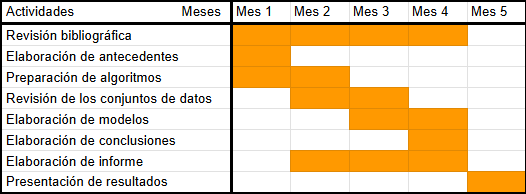
\includegraphics[width=0.8\linewidth]{cronograma.png}
    \caption{Diagrama de Gantt del proyecto. Las barras representan la duración planificada
de cada actividad; los rombos naranjas son los hitos principales y las flechas indican
relaciones de precedencia.}
    \label{fig:placeholder}
\end{figure}

\section{Índice propuesto}
\addcontentsline{toc}{section}{Índice propuesto}

\begin{enumerate}[leftmargin=2em]
    \item \textbf{Introducción}
    \begin{enumerate}[label=\arabic*.\arabic*.]
        \item Antecedentes y motivación
        \item Planteamiento del problema
        \item Hipótesis de trabajo
        \item Objetivos (general y específicos)
    \end{enumerate}
    \item \textbf{Marco teórico y estado del arte}
    \begin{enumerate}[label=\arabic*.\arabic*.]
        \item La depresión: definición clínica y epidemiológica
        \item Lingüística de la depresión: marcadores psicolingüísticos
        \item Procesamiento de Lenguaje Natural y transformers
        \item Aprendizaje automático supervisado y explicable
    \end{enumerate}
    \item \textbf{Datos}
    \begin{enumerate}[label=\arabic*.\arabic*.]
        \item Revisión de corpus públicos (\emph{MentalRiskES}, \emph{Leis et al.}, \emph{eRisk}, \emph{DAIC-WOZ})
        \item Construcción y anonimización del corpus propio
        \item Análisis exploratorio de datos (EDA)
    \end{enumerate}
    \item \textbf{Metodología}
    \begin{enumerate}[label=\arabic*.\arabic*.]
        \item Preprocesamiento y extracción de características
        \item Líneas base clásicas (TF-IDF + LR/SVM)
        \item Ajuste fino de BETO
        \item Modelo híbrido (embeddings + LIWC)
        \item Protocolo de evaluación y métricas
        \item Interpretabilidad (SHAP/LIME)
    \end{enumerate}
    \item \textbf{Resultados y discusión}
    \begin{enumerate}[label=\arabic*.\arabic*.]
        \item Comparación de modelos
        \item Análisis de errores y sesgos
        \item Limitaciones y amenazas a la validez
    \end{enumerate}
    \item \textbf{Conclusiones y trabajo futuro}
    \item \textbf{Bibliografía}
    \item \textbf{Anexos} (código, particiones, prompts, hojas de consentimiento)
\end{enumerate}

\newpage
\bibliographystyle{ieeetr}
\bibliography{references}

\end{document}
